\chapter{Future perspectives}\label{future}

This manuscript does not mark the end of the projects herein; the development of blik --- and of the ecosystem it lives in --- is ongoing, and much more is in the plans to further our understanding of \textit{D. radiodurans} and its key players, such as FtsZ and HU.

\localtableofcontents

\section{blik}

The development of blik has already proven useful for daily use in our group and others.
However, there are several features that were part of blik's original plan, but which are not yet implemented, or only partially.
Other planned enhancements are not specific to blik, but more general napari features which will benefit blik and hopefully many other plugins and applications depending on napari.

\subsection{STA visualisation \textit{in situ}}
One of the main ones is the ability to visualise subtomogram averages \textit{in situ}, positioned and oriented based on the particle picks they originated from.
While some tools that can do this exist~\cite{ermelArtiaXElectronTomography2022}, they are either not fully interactive (particles cannot be selected, moved around, or isosurface levels changed), limited in performance, or both.
In order to develop this feature, some changes need to be done to napari to allow instance-based mesh and volume rendering.
Some of these changes are already partially implemented, and there are plans to continue on this development in the coming months.
Developing a generalized framework for such rendering in napari will also benefit several other fields where rendering of high numbers of instances at high performance is needed (molecular dynamics, highly-multiplexed labeling, astrophysics).

\subsection{3D interactivity}
3D interactivity in blik can still be significantly improved; some features planned for this purpose are:

\begin{enumerate}[noitemsep]
    \item particle picking on 3D slicing planes, without need to switch to 2D for accurate depth selection
    \item more ergonomic controls for orientation selection of picked particles
    \item improved two-way interaction between feature plots and 3D view (coloring, classifying, selecting particles)
\end{enumerate}

\subsection{Multicanvas}
Another crucial improvement for napari (and therefore blik) which is underway and has been on my --- and on other napari developers' --- to-do list is \href{https://github.com/napari/napari/issues/5348}{full support for multicanvas}.
Especially for segmentation and annotation, having access two linked views of 2D and 3D visualisations can make a big difference in the ergonomics of a tool.


\section{napari}

This thesis was heavily influenced and shaped by my extended collaboration with the \href{https://napari.org/}{napari} project~\cite{thenaparicommunityNapariMultidimensionalImage2024} and its core developers and community~\cite{thenaparicommunityCommunityNapari2024}, whose values and goals for the development of scientific software strongly align with mine.

The napari community aims to provide a fast, user-friendly, hackable and reusable library and application for the visualization and annotation of n-dimen\-sional scientific imaging data.
It's built on top of the well-established and wide\-spread libraries at the core of the scientific python ecosystem (such as numpy and pandas), in order to allow seamless interactive visualization both programmatically and via graphical user interface.
Our committed effort to bridge many different imaging fields in order to share knowledge and resources has resulted in a steady influx of new contributors and users from various backgrounds, who ensured napari remains user-friendly, hackable, and powerful.

Due to the distributed and collaborative nature of community-driven open-source development --- especially of as large a project as napari --- it's a difficult (and futile) exercise to determine who "authored" a specific feature, and yet the steady contributions from newcomers shows that this approach to development is what many research developers seek.

Other developers do not directly contribute to napari, but develop plugins for it instead.
There are already \href{https://www.napari-hub.org/plugins?search=cryo+ET&sort=relevance&page=1}{many cryo-ET-focused plugins} that appeared independently, which build upon some of the groundwork contributed to napari by me as part of this thesis and by many other contributors.

The current \href{https://github.com/orgs/napari/projects/24/views/2?pane=info}{napari roadmap} is filled with exciting new features, and I expect that in the next few years the project will continue growing and expanding to new fields.


\section{Teamtomo}\label{teamtomo}

As another effort to go against the academia-machine, early on in my PhD, Alister Burt and I started the \href{https://teamtomo.org}{teamtomo} project, with the goal of creating a shared, open-source resource for cryo-ET developers, and to encourage the community to collaborate on the development of cryo-ET software within the python ecosystem.

While at first we were the only two people involved, at the time of writing almost 30 researchers and developers from several different groups around the world have contributed to libraries and tools in the \href{https://github.com/teamtomo}{teamtomo repositories}, and more are joining our montly meetings where we plan future concerted efforts.

With time, we aim to collect well-scoped and well-documented libraries that cover all the needs of a cryo-ET data processing pipeline, from simple ones like I/O utilities or cross-correlation, to more complex routines such as tilt-series alignment.
Some of these tools --- contributed by various developers --- are already available, such as \href{https://github.com/teamtomo/ttmask}{ttmask} for mask creation, \href{https://github.com/teamtomo/cryohub}{cryohub} for I/O, or \href{https://github.com/teamtomo/fidder}{fidder} for fiducial masking.


\section{\textit{D. radiodurans}: FtsZ, HU, and more}

The ongoing efforts on HU and FtsZ encountered technical challenges that so far prevented us from reaching high resolution and unraveling the structure and function of these proteins.
We already started to work around these challenges, and Harald Bernhard --- a joint GenOM/MICA postdoc --- has picked up the work on these projects and already started improving on it.
There are also new directions in which we'd like to extend our work on \textit{D. radiodurans}, using cryo-EM, cryo-ET and other imaging techniques; particularly, we're interested in understanding the effects of radiation damage on all these processes, and how \textit{D. radiodurans} protects itself from it.

\subsection{Chromatin and HU}\label{future_hu}

To increase our chances to identify and pick HU, a new dataset was collected with a phase plate, which allows to collect data closer to focus while improving the contrast of low spatial fequency information (\fullref{em_ctf}).
Preliminary results on this data showed more classes containing what could be HU in a similar conformation to what was seen in \figref{fig:hu_structure}, but more work is needed.

% TODO: any plans/ideas still for tomography here?

\subsection{FtsZ SPA}\label{future_ftsz_spa}

Since Harald picked up this project, he has already managed to improve the results from the FtsZ+DDM dataset in a few ways.
With careful use of 2D and 3D classifications, it's possible to better isolate single filaments, which improves the initial model generation.
Balancing the different views by number of particles also improves the orientation distribution, reducing map artifacts at the cost of some global resolution.
Additionally, the use of a bigger box size in particle extraction has improved slightly the quality of the alignements and 2D class averages.
While the anisotropy issue remains, the new maps are much more interpretable, and match quite well those by \citet{fujitaStructuresFtsZSingle2023} from \textit{K. pneumoniae} FtsZ (\figref{fig:ftsz_hari_map}).

\begin{figure}
    \centering
    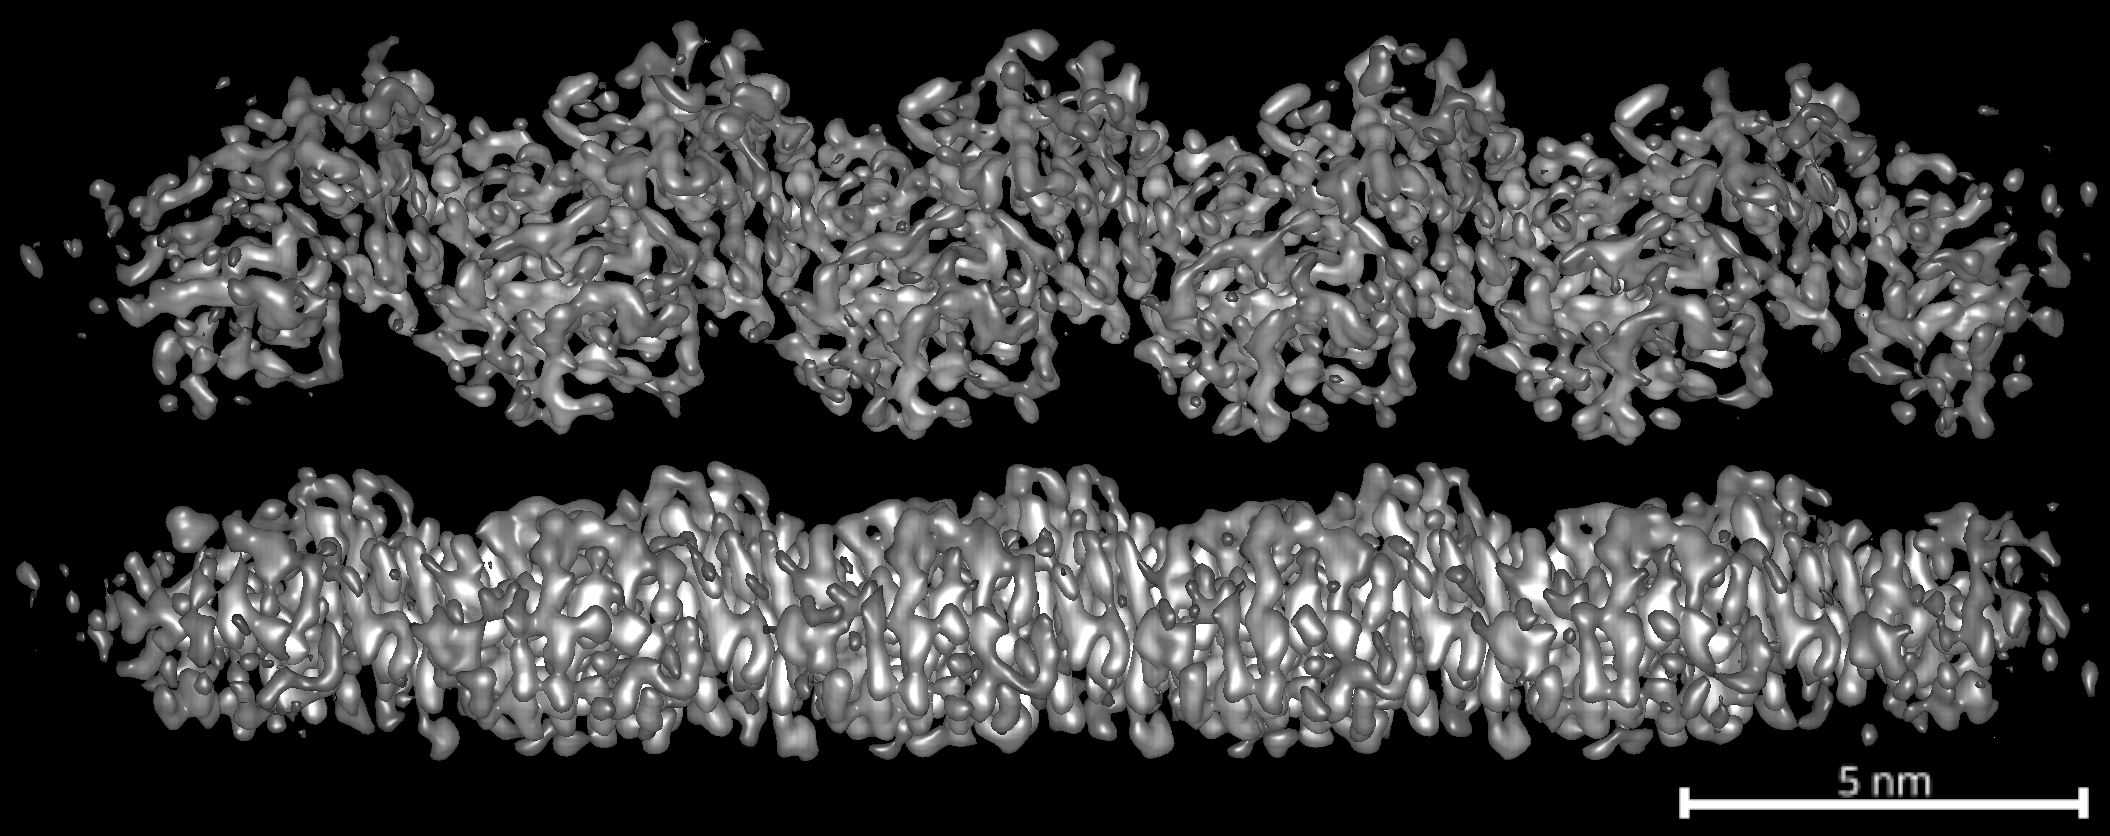
\includegraphics[width=\textwidth]{other/ftsz_map_good.png}
    \titledcaption[3D map of FtsZ with detergent]{Using the FtsZ+DDM dataset, and more careful 2D and 3D classifications to clean the dataset and better balance different views, Harald significantly improved on the FtsZ filament map. Preferential orientation is unfortunately still not fully solved, as evidenced by the streaking artifacts along one direction (bottom view), which are not present in the other (top view).}
    \label{fig:ftsz_hari_map}
\end{figure}

Depending on the outcome of the detergent dataset, we might need to go back to the tilted dataset.
We think that the process of assigning angles and restricting the search should be theoretically sound, so it may be worth spending more time tweaking parameters in Relion to find a working setup.
A recent study by ~\citet{aiyerOvercomingResolutionAttenuation2024} showed that negative effects of thickening the sample (due to tilting) should be negligible with proper preprocessing, so the achievable resolution should be unrestricted by the tilt.

\subsection{FtsZ STA}\label{future_ftsz_sta}

The cryo-ET dataset used in the septation paper (\fullref{drad}) was collected with the goal of capturing a wide field of view including a full \textit{D. radiodurans} cell.
For this reason, it contains a relatively low amount of FtsZ bundles (which are often not visible and/or not present in the lamellae), and has a relatively high pixel size (4.346 Å/px), which significantly limits our ability to reach high resolutions.

A new dataset has recently been collected by Harald with higher magnification and focused on the septa tips, which will hopefully provide a higher resolution view on the tips.

However, another problem with STA of FtsZ was the preferential orientation of the filaments, a consequence of how \textit{D. radiodurans} lies on the grid.
A way to tackle this problem is to force the bacteria into different orientations, for example by creating a dense paste of bacteria to freeze using the waffle method~\cite{kelleyWaffleMethodGeneral2022}.
Preliminary attempts to prepare such sample were promising, but due to technical problems with the cryo-FIB microscope we were not yet able to continue with this sample.
Similarly, freezing the sample with a Leica™ plunge freezer showed a more diverse orientation distribution of the bacteria.

\subsection{Effects of stress and radiation}

\textit{D. radiodurans} is especially intriguing due its incredibly effective radiation and stress resistance machinery.
While the FtsZ and HU projects are interesting by themselves, they all fit in a wider question: \textbf{How does \textit{D. radiodurans} protect itself from radiation?}
To answer this, we plan to compare how the known machineries are affected by radiation exposure.
Some preliminary cryo-ET data, collected at the same time as the septation dataset (\fullref{drad}), appeared to show some morphological differences in the nucleoid and membranes after irradiation.
New, higher magnification data will probably be collected to move this investigation further.

\subsubsection{Structural proteomics}

The study of the effects of radiation damage on \textit{D. radiodurans} may come in the form of another cross-over with the cell-extract project in the MICA group (\fullref{emscan}).
Cell-extract SPA cryo-EM could be used to perform \textbf{structural proteomics}, identifying not only the changes in the proteome caused by irradiation, but the effects that these have on protein structures and complexes.


\section{Cryo-ET}

During the course of this thesis, the cryo-ET world has changed a lot, starting from improved sample preparation techniques, all the way to high resolution STA processing and post-processing.

\subsection{Hardware}

Cryo-FIB milling~\cite{markoFocusedionbeamThinningFrozenhydrated2007} has become an essential procedure in every group working on cellular tomography, leading to the automation of lamellae production being a major focus of hardware and software development around the world.
The combination of FIB milling and Correlative light-electron microscopy (CLEM) is especially powerful, pushing the field towards being able to reliably and accurately locate a structure of interest in a large cell or tissue, cut out a lamella, and image it at high resolution~\cite{bergerCryoelectronTomographyFocused2023,debeerPreciseTargeting3D2023,klumpeModularPlatformAutomated2021}.

Exciting progress is being made towards cheaper, smaller, lower-energy microscopes that are still powerful and capable of high resolution work~\cite{naydenovaCryoEM100KeV2019,russoElectronCryomicroscopeHardware2023} --- though for thicker samples it might be more complicated (\figref{fig:et_smallest_particle}).
Development of such instruments will hopefully help spread and democratize electron-microscopy, which currently requires extremely expensive equipment (due also in part to the quasi-monopolistic industry) and is therefore in constant lack of supply and out of reach for many researchers around the world.


\subsection{Software}

During the course of this thesis, many new software suites and standalone tools have appeared, improving the field both in ergonomics and algorithmically.

Software pipelines are steadily moving away from the naive "reconstruct full tomogram -> extract subvolumes" approach in favour of different flavours of per-particle tilt-series, as the field pushes for sub-nanometer resolution.

Interactive visualization tools like blik~\cite{gaifasBlikExtensible3D2024} and ArtiaX~\cite{ermelArtiaXElectronTomography2022} appeared to answer the need for a HITL workflow, together with integrative workflow managers like Scipion~\cite{delarosa-trevinScipionSoftwareFramework2016} now providing extensive support for cryo-ET.

Community initiatives --- such as Teamtomo --- aiming to establish common frameworks and conventions will be paramount to the development of the cryo-ET software ecosystem.

The field giant Relion has implemented an almost full pipeline for cryo-ET and STA~\cite{zivanovBayesianApproachSingleparticle2022,burtImageProcessingPipeline2024}, and many other complete software suites are being published, often together with novel and unique tools~\cite{balyschewStreamlinedStructureDetermination2023,galaz-montoyaSingleParticleTomography2015,galaz-montoyaAlignmentAlgorithmsPerparticle2016,himesEmClaritySoftwareHighresolution2018,liuNextPYPComprehensiveScalable2023}.

Of note is also the recently (beta) release of \href{https://github.com/warpem/warp}{Warptools}, a linux port of Warp~\cite{tegunovRealtimeCryoelectronMicroscopy2019} allowing to finally integrate parts of the Warp pipeline into others, without the need of using a graphical interface and a Windows machine.

The tide of Machine-learning tools of the last few years has flooded --- among many others --- the cryo-ET field, giving rise to powerful automated tools for denoising~\cite{beplerTopazDenoiseGeneralDeep2020}, segmentation~\cite{lammMemBrainV2Endtoend2024,eisensteinSmartParallelAutomated2024}, picking~\cite{wagnerEvolutionSPHIREcrYOLOParticle2020,riceTomoTwinGeneralized3D2023}, modeling~\cite{jamaliAutomatedModelBuilding2024}, structure prediction~\cite{jumperHighlyAccurateProtein2021,abramsonAccurateStructurePrediction2024,baekAccuratePredictionProtein2021}, and much more.
While these tools may work like magic, it's important to keep an eye out for hallucinations~\cite{maynezFaithfulnessFactualityAbstractive2020}, especially as the field moves towards heavier and more normalized use of the technology; ML validation and introspection are already a high priority in other fields, and cryo-ET will be no exception.

\subsection{Applications}

As cryo-ET becomes more widespread, it's being used in a variety of different and novel applications; with this wider spectrum of literature, the community is realizing where cryo-ET really shines, and where other techniques might be preferrable.
Especially thanks to the evolution of FIB milling and the ever faster data collection, high-resolution structure determination \textit{in situ} can also be achieved by using SPA on the same samples (with all the SNR benefit that comes with it).
On the other hand, cryo-ET is establishing as the go-to technique for superstructural studies, where the mesoscale view allows to investigate emergent structures and behaviours which are simply too heterogeneous to be visible via SPA.

A particularly exciting prospect for me is the marriage of cryo-ET and (coarse-grained) molecular dynamics to investigate large systems such as whole cells, which was only dreamed of at the beginning of my thesis~\cite{earnestChallengesIntegratingStochastic2017}.
The cryo-ET/MD combination is already bearing fruits in exploring conformational variability~\cite{vuillemotMDTOMOMethodContinuous2023}, in multi-scale modeling~\cite{liDevelopmentMultiscaleUltracoarsegrained2023}, and much more; it's only a matter of time before we'll be able to take a snapshot of a cell \textit{in situ}, and just simulate to see what happens next.
